% Build: app/build_paper.sh (XeLaTeX via Tectonic). The official ACL style files are downloaded at
% build time from a pinned commit; they are not modified. "review" prints an anonymous submission with
% line numbers; switch to "preprint" (named authors, page numbers) once the author block is filled in.
\documentclass[11pt]{article}
\usepackage[review]{acl}
\usepackage{microtype}

% Fonts: Times-like Latin and math (TeX Gyre Termes) with Noto Serif KR for Hangul.
\usepackage{amsmath}
\usepackage{unicode-math}
\setmainfont{texgyretermes}[Extension=.otf, UprightFont=*-regular, BoldFont=*-bold,
  ItalicFont=*-italic, BoldItalicFont=*-bolditalic]
\setmathfont{texgyretermes-math.otf}
\setmonofont{Inconsolatazi4-Regular.otf}[BoldFont=Inconsolatazi4-Bold.otf, Scale=0.92]
\usepackage{kotex}
\setmainhangulfont{NotoSerifKR}[Path=.build/fonts/, Extension=.otf, UprightFont=*-Regular,
  BoldFont=*-Bold, ItalicFont=*-Regular, BoldItalicFont=*-Bold, Scale=0.94]
\setsanshangulfont{NotoSerifKR}[Path=.build/fonts/, Extension=.otf, UprightFont=*-Regular,
  BoldFont=*-Bold, Scale=0.94]
\setmonohangulfont{NotoSerifKR}[Path=.build/fonts/, Extension=.otf, UprightFont=*-Regular,
  BoldFont=*-Bold, Scale=0.94]

\usepackage{graphicx}
\usepackage{booktabs}
\usepackage{enumitem}
\usepackage{array}

% Korean names for the fixed headings of the ACL style.
\renewcommand{\abstractname}{초록}
\renewcommand{\figurename}{그림}
\renewcommand{\tablename}{표}
\renewcommand{\appendixname}{부록}
\makeatletter
\def\thebibliography#1{\vskip\parskip\vskip\baselineskip\def\baselinestretch{1}%
  \ifx\@currsize\normalsize\@normalsize\else\@currsize\fi\vskip-\parskip\vskip-\baselineskip
  \section*{참고문헌\@mkboth{참고문헌}{참고문헌}}\list{}{\setlength{\labelwidth}{0pt}%
  \setlength{\leftmargin}{\parindent}\setlength{\itemindent}{-\parindent}}%
  \def\newblock{\hskip .11em plus .33em minus -.07em}%
  \sloppy\clubpenalty4000\widowpenalty4000\sfcode`\.=1000\relax}
\makeatother

\newcommand{\pp}{\%p}

\title{골든셋의 라벨 오류는 모델 선택 결정을 얼마나 바꾸는가:\\
MMLU-Redux 자연 실험, 오류 주입, 선행 연구 결과와의 비교}

\author{저자 정보는 심사용 익명 원고에서 생략}

\begin{document}
\maketitle

\begin{abstract}
모델 교체나 배포 결정은 흔히 골든셋에서 측정한 두 모델의 점수 차이에 근거한다. 골든셋에 라벨 오류가 흔하다는 보고는 많지만, 이 오류가 모델 쌍의 비교 결정을 얼마나, 어느 방향으로 바꾸는지는 정량화되지 않았다. 본 연구는 공개 모델 42종의 MMLU 문항별 예측과 MMLU-Redux 2.0의 전문가 수정 정답으로 자연 실험과 오류 주입 실험을 수행하고, 선행 연구 여섯 편의 분석을 같은 자료에서 재현하거나 대응 값을 계산하여 그 보고값과 비교하였다. 외부에서 받은 모델 예측은 세 모델을 직접 다시 실행하여 검증하였다. 전체 평가셋에서는 라벨 수정으로 바뀐 결정이 드물었으나, 과목 단위의 작은 평가셋에서는 수정 문항이 많을수록 반전이 많았고 바이러스학에서는 결정의 36\%가 바뀌었다. 실제 오류 수준에서 우세 방향이 뒤집힌 경우는 없었으며, 라벨 오류는 모델 간 격차를 줄여 결정을 보류로 바꾸었다. 어려운 문항에 모델들이 가장 많이 고르는 오답을 표시하는 체계적 오류는 무작위 오류보다 결정을 1.4--1.6배 많이 바꾸었다. 선행 연구와 비교하면 MMLU-Redux의 오류율은 판단 유보 문항을 빼면 재현되었으나, 오류 문항을 빼고 채점하는 선행 연구의 비교를 적용하면 같은 수의 문항을 무작위로 뽑기만 해도 비슷한 크기의 순위 변화가 생겼다. 또한 이미지 분류에서 보고된 것과 달리 성능이 높은 모델일수록 오류 문항에서 수정 정답을 더 자주 골라, 라벨 오류는 강한 모델에 불리하게 작용하였다. 골든셋의 허용 오류율은 체계적 오류를 가정하여 정하고, 작은 평가셋과 오류가 몰린 하위 집합은 따로 감사할 필요가 있다.
\end{abstract}

{\renewcommand{\abstractname}{Abstract}
\begin{abstract}
Model replacement and deployment decisions often rest on the score difference between two models on a golden evaluation set. Label errors in such sets are common, yet how much they change pairwise model-selection decisions, and in which direction, has not been quantified. Using per-item MMLU predictions from 42 open models and the expert corrections of MMLU-Redux 2.0, we run a natural experiment and a controlled injection experiment, and we replicate the analyses of six prior studies on the same data, or compute matching quantities, to compare their reported values with ours. We verify the third-party predictions by re-running three of the models ourselves. On the full set, correcting labels rarely changed a decision. On small subject-level sets, flips grew with the share of corrected items and reached 36\% of decisions in virology. At real error levels no decision reversed the winner. Instead, label errors compressed the gaps between models and turned decisions into inconclusive ones. Systematic errors, which label hard items with the distractor most models choose, changed 1.4--1.6 times as many decisions as random errors. Against prior work, the MMLU-Redux error rate replicated once items the annotators left undecided are set aside, but applying the earlier comparison that scores only error-free items produced rank changes of a similar size when the same number of items was simply drawn at random. Unlike in image classification, stronger models chose the corrected answer on erroneous items more often, so label errors worked against the strongest models. Error tolerances for golden sets should assume systematic errors, and small sets and error-dense subsets need their own audits.
\end{abstract}}

\section{서론}

LLM 애플리케이션을 운영하는 팀은 새 모델이나 프롬프트의 도입 여부를 정할 때 고정된 평가 데이터셋, 즉 골든셋에서 후보와 현재 모델의 점수를 비교한다. 이때의 결정은 대개 ``후보 $B$가 현재 모델 $A$보다 $\delta$ 이상 낫다''는 쌍 비교의 형태를 띤다. 골든셋의 정답 라벨이 틀리면 이 비교의 근거도 함께 흔들린다.

공개 평가셋의 라벨 오류는 드물지 않다. 널리 쓰이는 시험셋 10종에서는 평균 3.3\% 이상의 라벨 오류가 발견되었고, 수정한 라벨로 평가해도 전체 순위는 거의 그대로였으나 오류 문항의 비율이 몇 \%p만 높아져도 순위가 바뀔 수 있었다\citep{northcutt2021pervasive}. MMLU\citep{hendrycks2021mmlu}는 문항의 약 6.5\%에 오류가 있는 것으로 추정되었으며\citep{gema-etal-2025-done}, 라벨 오류와 모호한 문항을 걷어 낸 벤치마크에서도 최신 모델이 단순한 문항에서 여전히 실패하였다\citep{vendrow2025platinum}.

평가 결론의 불확실성에 관한 연구는 주로 표본 변동과 검정력을 다루었다\citep{card-etal-2020-little,madaan2024variance}. 라벨 오류의 양과 종류가 쌍 비교 결정을 얼마나, 어느 방향으로 바꾸는지를 표본 변동과 분리하여 측정한 연구는 찾기 어렵다. 골든셋의 구축과 검증을 다룬 선행 리뷰\citep{anonymous2026review}도 이를 연구 공백으로 꼽았다. 선행 연구들이 보고한 오류율과 순위 변화도 서로 다른 모델과 절차에서 나온 값이어서, 같은 자료에서 비교하면 어떻게 되는지는 확인되지 않았다. 이 리뷰는 맹검 감사의 통과 기준으로 ``오류율의 95\% Wilson 상한이 $\delta/4$ 이하''를 제안하였으나, 이 기준을 뒷받침하는 실증 결과는 없었다.

본 연구는 세 실험으로 이 공백을 다룬다. 첫째는 MMLU-Redux 2.0의 전문가 재주석을 이용한 자연 실험이다. 공개 모델 42종의 문항별 예측에 원래 정답과 수정 정답을 각각 적용하여 두 조건의 쌍 비교 결정을 비교한다. 둘째는 오류 주입 실험이다. 오류를 넣을 문항과 잘못된 라벨의 종류를 따로 바꾸어 오류 메커니즘의 효과를 분리하고, 라벨은 그대로 두고 문항만 바꾸는 기준선과 비교한다. 셋째는 선행 연구의 재현이다. 선행 연구 여섯 편의 분석을 같은 자료에서 재현하거나 대응 값을 계산하여 그들의 보고값과 본 연구의 측정값을 나란히 놓고, 차이가 생기는 원인을 따진다. 외부에서 받은 모델 예측은 세 모델을 다시 실행하여 검증한다. 연구 질문은 다음 다섯 가지이다.

\begin{enumerate}[label=\textbf{RQ\arabic*.}, leftmargin=*, itemsep=1pt, topsep=3pt]
\item 실제 라벨 오류를 수정하면 쌍 비교 결정은 얼마나 바뀌는가?
\item 실제 라벨 오류는 무작위로 생기는가, 아니면 모델들이 고르는 오답 쪽으로 치우치는가?
\item 결정 반전은 오류율, 오류 메커니즘, 평가셋 크기에 따라 어떻게 달라지며, 라벨 오류 없이 문항만 바꾼 경우와 비교하면 어떠한가?
\item $\delta/4$ 감사 기준은 어느 정도의 오류율을 걸러내며, 그 경계의 오류율에서 결정은 얼마나 안정적인가?
\item 선행 연구가 보고한 오류율, 순위 변화, 평가 잡음의 크기는 같은 자료에서 재현한 본 연구의 값과 일치하는가? 다르다면 그 차이는 어디서 오는가?
\end{enumerate}

주요 결과는 네 가지이다. 첫째, 라벨 오류는 실제 오류 수준과 주입 실험의 어느 조건에서도 우세 방향을 뒤집지 않았고, 모델 간 격차를 줄여 결정을 보류로 바꾸었다. 둘째, 무작위 라벨 오류의 영향은 같은 수의 문항을 교체할 때와 비슷하였다. 어려운 문항에 모델들이 가장 많이 고른 오답(이하 대표 오답)을 표시하는 체계적 오류는 무작위 오류보다 결정을 1.4--1.6배 많이 바꾸었고, 실제 오류도 대표 오답 쪽으로 치우쳐 있었다. 셋째, 선행 리뷰의 감사 기준이 허용하는 경계 오류율(0.75\%)에서도 870문항 평가셋의 결정 반전율은 1\% 안팎이었다. 넷째, 선행 연구와 비교하면 MMLU-Redux의 오류율은 재현되었으나, 오류 문항을 빼고 채점할 때의 순위 변화는 같은 수의 문항을 무작위로 뽑아도 비슷하게 생겼다. 또한 이미지 분류에서 고용량 모델이 틀린 라벨을 더 따른다는 보고와 달리, 성능이 높은 LLM일수록 오류 문항에서 수정 정답을 더 자주 골랐다.

\section{관련 연구}

\paragraph{평가셋의 라벨 오류.}
\citet{northcutt2021pervasive}의 연구는 confident learning으로 오류 후보를 찾고 크라우드소싱으로 확인하여 시험셋 10종의 라벨 오류를 추정하였다. MMLU-Redux\citep{gema-etal-2025-done}는 MMLU 문항을 전문가가 다시 주석하고, 오류를 정답 오류, 질문 불명확, 복수 정답 등의 유형으로 나누었다. \citet{vendrow2025platinum}의 연구는 여러 벤치마크에서 라벨 오류와 모호한 문항을 제거한 판을 만들어 모델의 신뢰성을 다시 평가하였다. 이 연구들은 오류의 빈도와 순위 변화를 보고하였으나, 실무에서 쓰는 쌍 비교 결정이 얼마나 바뀌는지는 측정하지 않았다. 5절에서는 이 연구들의 분석을 같은 자료에 재현하여 보고값과 비교한다.

\paragraph{평가 결론의 통계적 불확실성.}
\citet{card-etal-2020-little}의 연구는 NLP 실험의 상당수가 작은 차이를 검출하기에 검정력이 부족함을 보였고, \citet{madaan2024variance}의 연구는 학습 시드에 따른 벤치마크 점수의 분산을 측정하였다. \citet{alzahrani-etal-2024-benchmarks}의 연구는 선택지 순서나 답 기호 같은 평가 형식의 작은 변화만으로 MMLU 순위가 크게 바뀜을 보였다. 이 연구들이 다룬 불확실성은 표본, 학습 과정, 평가 형식의 변동에서 온다. 본 연구는 같은 표본 안에서 라벨만 바꾸어, 라벨 오류의 효과를 표본 변동과 분리하여 측정한다.

\section{데이터와 방법}

\subsection{데이터}
MMLU-Redux 2.0\citep{gema-etal-2025-done}은 MMLU의 57과목에서 과목마다 100문항을 다시 주석한 자료이며, 문항마다 오류 유형과 정답 오류인 경우의 수정 정답을 제공한다. 모델 예측은 Open LLM Leaderboard v1\citep{beeching2023leaderboard}이 공개한 MMLU 5-shot 문항별 결과에서 가져왔다. 리더보드는 lm-evaluation-harness\citep{gao2023harness}로 네 선택지의 로그확률을 계산하며, 본 연구는 로그확률이 가장 큰 선택지를 모델의 예측으로 삼았다. 두 자료는 과목명과 프롬프트 문자열을 키로 결합하였다(부록~\ref{app:details}). 5,700문항 중 5,690문항이 결합되었고, 리더보드에 정답이 기록된 문항에서 리더보드의 정답과 Redux의 원래 정답은 모두 일치하였다.

모델은 MMLU 문항별 결과가 공개된 2023--2024년의 공개 모델 42종이다(부록~\ref{app:models}). 후보 48종 가운데 6종은 문항별 결과를 얻지 못해 제외하였다. 3종은 추정한 이름의 리더보드 저장소가 없었으며, 이 중 OLMo는 실제 저장소 이름을 확인하여 두 모델(OLMo-7B-hf, OLMo-1.7-7B-hf)로 대체하였다. 나머지 3종인 Llama-2 chat 모델은 리더보드가 MMLU 문항별 결과를 공개하지 않았다.

본 연구는 모델을 새로 학습하거나 문항을 새로 주석하지 않았다. 정답 라벨과 수정 정답은 MMLU-Redux 주석자의 판단이고, 모델 예측은 리더보드가 계산한 로그확률이다. 이 두 외부 자료 위에서 문항 결합, 결정 반전 계산, 오류 주입, 감사 계산, 선행 연구 분석의 재현은 모두 본 연구의 코드로 수행하였다. 외부 예측을 그대로 믿지 않기 위해 세 모델은 이 연구의 컴퓨터에서 다시 실행하여 리더보드의 예측과 비교하였다(\ref{sec:method-compare}절).

\subsection{라벨 조건}
Redux 주석에 따라 문항을 세 범주로 나누었다. 오류가 없는 문항(5,321문항), 정답 오류로 표시되고 원래 정답과 다른 수정 정답이 명시된 수정 가능 문항(100문항), 그리고 그 밖의 오류가 있는 미해결 문항(269문항)이다. 미해결 문항에는 질문이 불명확하거나 정답이 여럿이어서 정답 하나로 고칠 수 없는 문항이 포함된다.

오류가 없는 문항과 수정 가능 문항을 합친 5,421문항을 분석 집합 $S$라 하고, $S$의 수정 정답을 기준 라벨로 삼았다. 관측 라벨은 두 가지이다. 첫째는 $S$의 원래 정답으로, 기준 라벨과의 차이는 라벨 오류의 효과만 반영한다. 둘째는 결합된 5,690문항 전체의 원래 정답으로, 리더보드의 공개 점수와 같은 조건이다. 이 조건에는 라벨 오류의 효과와 미해결 문항이 포함된 효과가 함께 들어 있다. 과목별 수정 문항 비율은 그 과목의 $S$ 문항 중 수정 가능 문항이 차지하는 비율로 정의하였으며, Redux가 보고한 과목별 오류율과는 다르다.

\subsection{결정 규칙과 결정 반전}
모델 쌍 $(A, B)$마다 같은 문항에서의 정확도 차이 $d = \mathrm{acc}_B - \mathrm{acc}_A$와 그 95\% 신뢰구간 $[L, U]$를 계산하였다. 신뢰구간은 문항별 정답 여부의 쌍체 분산을 이용한 정규근사로 구하였다. 결정 여유 $\delta$에 대해, $d \ge \delta$이고 $L > 0$인 쌍은 $B$ 우세, $d \le -\delta$이고 $U < 0$인 쌍은 $A$ 우세로 판정하고, 나머지 쌍은 보류로 판정하였다.
$\delta$로는 0, 1, 2, 3, 5\pp{}를 사용하였고, 본문에는 선행 리뷰의 예시와 같은 3\pp{}의 결과를 주로 보고한다. 민감도 분석으로, 신뢰구간 대신 정확 McNemar 검정\citep{mcnemar1947note}의 $p$값에 861쌍 전체에 대한 Holm 보정\citep{holm1979simple}을 적용한 규칙도 계산하였다.

기준 라벨과 관측 라벨에서 판정이 다르면 결정이 반전되었다고 한다. 반전은 세 가지로 나눈다. 기준에서 우세였던 쌍이 보류가 되는 결정 상실, 보류였던 쌍이 우세가 되는 허위 결정, 우세 방향이 뒤바뀌는 역전이다. 반전율은 반전된 쌍의 수를 전체 쌍의 수로 나눈 값이다.

\subsection{오류 주입}
$S$에서 $n$문항($n$ = 100, 300, 870, 5,421)을 비복원 추출해 골든셋을 만들고, 기준 라벨로 내린 판정과 오류를 넣은 라벨로 내린 판정을 비교하였다. 오류 문항 수는 $k \sim \mathrm{Binomial}(n, e)$로 뽑았다. 작은 평가셋에서는 $ne$가 1보다 작을 수 있으므로, $k$를 이항분포에서 뽑아 반복 평균의 오류율이 $e$가 되게 하였다. 오류율은 0.25\%부터 12\%까지 아홉 수준을 사용하였다. 870문항은 선행 리뷰가 $\delta$ = 3\pp{}, 두 모델의 정오가 엇갈린 문항 비율 0.10, 검정력 80\%를 가정해 권한 골든셋 크기이다.

\begin{table}[t]
\centering\small
\begin{tabular}{@{}lll@{}}
\toprule
조건 & 문항 선택 & 변경 내용 \\
\midrule
무작위 오류 & 균일 & 무작위 오답 라벨 \\
대표 오답 오류 & 균일 & 대표 오답 라벨 \\
어려운 문항 오류 & 오답률 비례 & 무작위 오답 라벨 \\
체계적 오류 & 오답률 비례 & 대표 오답 라벨 \\
\midrule
문항 교체 기준선 & 균일 & 표본 밖 문항으로 교체 \\
문항 제거 기준선 & 균일 & 문항 제거 \\
\bottomrule
\end{tabular}
\caption{오류 주입 조건. 모든 조건은 $k$개 문항을 바꾼다. 오답률과 대표 오답은 평가 대상이 아닌 다른 모델 집단에서 계산한다.}
\label{tab:conditions}
\end{table}

오류 메커니즘은 두 요인을 교차한 네 조건이다(표~\ref{tab:conditions}). 첫째 요인은 오류를 넣을 문항의 선택으로, 균일 추출과 문항별 오답률에 비례한 추출이 있다. 오답률에 비례한 추출은 모델이 자주 틀리는 어려운 문항을 더 많이 고른다. 둘째 요인은 새 라벨로, 세 오답 중 하나를 균등하게 고르는 무작위 오답과 대표 오답이 있다. 대표 오답이 여럿이면 선택지 순서가 앞선 것을 택하였다. 어려운 문항을 골라 대표 오답을 표시하는 조건을 체계적 오류라 부른다.

평가 대상 모델의 예측으로 대표 오답을 정하면, 그 모델이 고른 오답이 정답으로 표시되어 그 모델이 유리해진다. 이를 피하기 위해 교차 적합을 사용하였다. 모델 42종을 무작위로 21종씩 두 집단으로 나누고, 한 집단 안의 쌍(210쌍)을 평가할 때는 대표 오답과 문항별 오답률을 다른 집단의 모델에서 계산하였다.

라벨 오류가 없는 교란과 비교하기 위해 기준선 두 가지를 두었다. 문항 교체 기준선은 같은 수 $k$의 문항을 표본 밖의 $S$ 문항으로 바꾸고, 문항 제거 기준선은 $k$개 문항을 뺀다. 전체 평가셋에서는 바꿀 문항이 남지 않으므로 교체 기준선을 계산하지 않았다.

모든 조건은 같은 표본에서 기준 라벨로 내린 판정과 비교하므로, 반전율은 표본 추출 변동을 포함하지 않는다. 반복은 평가셋 크기마다 300회(전체 평가셋은 60회)이다. 반전율에는 반복 간 95\% 신뢰구간을, 조건 간 배율에는 반복 단위 부트스트랩(1,000회) 95\% 신뢰구간을 붙였다. 세부 사항은 부록~\ref{app:details}에 정리하였다.

\subsection{그 밖의 분석}
RQ2에서는 수정 가능 100문항의 원래 정답이 모델 42종 전체의 대표 오답과 일치하는 비율을 우연 기댓값 1/3과 단측 이항검정으로 비교하였다. 순위의 변화는 Kendall $\tau$\citep{kendall1938new}로 측정하였다. RQ4에서는 $m$문항 감사에서 오류가 0건일 때의 95\% Wilson 상한 $z^2/(m+z^2)$\citep{wilson1927probable}과 감사 통과 확률 $(1-e)^m$을 계산하였다($z$ = 1.96).

\subsection{선행 연구 분석의 재현}
\label{sec:method-compare}
RQ5를 위해 선행 연구의 분석을 본 연구의 모델 42종에서 재현하였다. 절차를 그대로 옮길 수 없는 경우에는 대응하는 값을 계산하였으며, 아래에서 그 차이를 밝힌다. 보고값은 각 논문의 본문, 표, 그림에서 옮겼으며, 출처 쪽수와 함께 코드 저장소의 한 파일에 모았다(부록~\ref{app:details}).

\paragraph{외부 예측의 재실행.} 리더보드 상세 파일에는 문항마다 모델에 넣은 5-shot 프롬프트의 토큰과 네 선택지 토큰의 로그우도가 저장되어 있다. 세 모델(phi-2, StableLM-3B-4E1T, Mistral-7B-v0.1)에 같은 토큰을 넣어 Transformers\citep{wolf2020transformers}로 로그우도를 다시 계산하고 리더보드의 값과 문항별로 비교하였다. 정밀도는 리더보드와 같은 float16을 썼고, 가중치는 현재 공개된 판을 썼다. 과목마다 같은 5-shot 앞부분은 한 번만 계산해 재사용하였다.

\paragraph{\citet{gema-etal-2025-done}.} 첫째, 배포된 MMLU-Redux 2.0 주석으로 과목별 오류 유형의 수를 다시 세고, MMLU 과목 크기로 가중한 층화 추정치를 논문의 표와 비교하였다. 둘째, 그들은 상위 10개 모델의 순위를 HELM의 전체 문항 점수와 Redux의 오류 없는 문항 점수로 비교하였다. 같은 비교를 모델 42종에 적용하고, 라벨과 무관한 변화를 보기 위한 대조 두 가지를 두었다. 하나는 과목의 MMLU 전체 문항에서 오류 없는 문항과 같은 수의 문항을 무작위로 뽑는 것이고, 다른 하나는 Redux의 100문항에서 오류 문항과 같은 수의 문항을 무작위로 빼는 것이다(각 200회). 셋째, 모델마다 과목별 정확도와 과목의 오류 없는 문항 비율 사이의 Pearson 상관을 계산하였다.

\paragraph{\citet{vendrow2025platinum}.} 모델 오답 가운데 벤치마크 오류가 차지하는 몫을, 평가셋을 정제한 뒤 줄어든 평균 오답 수의 비율로 계산하였다. 정제는 미해결 문항을 빼고 수정 가능 문항의 라벨을 고치는 것이다.

\paragraph{\citet{northcutt2021pervasive}.} 그들의 정의에 따라 수정 가능 문항을 $C$(100문항), 오류가 없는 문항을 $B$(5,321문항)로 두고 미해결 문항은 제외하였다. 오류 문항의 비율은 $N = |C|/(|C|+|B|)$이며 원래 값은 $N_0$ = 1.84\%이다. $B$의 문항을 무작위로 줄여 $N$을 높이면 모델의 기대 정확도는 $N A_C + (1-N) A_B$가 된다. $A_C$와 $A_B$는 $C$와 $B$에서의 정확도이다. $N$에 따라 원래 라벨과 수정 라벨에서 쌍의 순서가 바뀌는 비율을 구하고, $B$를 실제로 줄인 평가셋(200회 반복)에 본 연구의 결정 규칙을 적용하였다. 모델 용량의 효과는 $A_B$와, $C$에서 원래의 틀린 라벨을 고른 비율 사이의 Spearman 상관으로 보았다. 그들의 모델은 같은 분포의 잡음이 섞인 학습 라벨로 학습되었지만, 본 연구의 LLM은 그렇지 않다는 차이가 있다.

\paragraph{평가 잡음과의 비교.} \citet{madaan2024variance}의 100문항 부분셋 결과에 대응하여, $S$에서 무작위로 뽑은 100문항(300회)과 전체 $S$ 사이에 순서가 바뀌는 쌍의 비율을 계산하였다. 그들의 값은 IRT로 고른 100문항의 가중 추정치이므로 무작위 표본과 절차가 다르다. \citet{card-etal-2020-little}와 비교하기 위해 검정력 80\%의 최소 검출 효과를 쌍마다 $(z_{0.975}+z_{0.8})\,\sigma_d/\sqrt{n}$으로 계산하였다. $\sigma_d$는 두 모델의 문항별 정오 차이의 표준편차로, 그들은 회귀로 예측한 일치율을 썼지만 본 연구는 관측값을 썼다. \citet{alzahrani-etal-2024-benchmarks}와는 순위가 바뀐 모델의 수와 최대 이동 폭을 비교하였다.

\section{결과}

\subsection{실제 오류를 고쳐도 순위는 유지되었고, 반전은 작은 평가셋에 몰렸다}
\label{sec:natural}

\begin{table}[t]
\centering\small\setlength{\tabcolsep}{4.2pt}
% generated by app/tables.py from results/; do not edit by hand
\begin{tabular}{@{}lrrrrr@{}}
\toprule
조건 & 기준 우세 & 반전 & 상실 & 허위 & 역전 \\
\midrule
\multicolumn{6}{@{}l}{\textit{전체 평가셋, 861쌍}} \\
$S$의 원래 정답 & 735 & 8 & 2 & 6 & 0 \\
공개 점수 & 735 & 10 & 5 & 5 & 0 \\
McNemar--Holm & 735 & 8 & 2 & 6 & 0 \\
\midrule
\multicolumn{6}{@{}l}{\textit{과목 단위 평가셋, 57과목, 49,077쌍}} \\
$S$의 원래 정답 & 26,851 & 1,086 & 764 & 322 & 0 \\
McNemar--Holm & -- & 447 & -- & -- & 0 \\
\bottomrule
\end{tabular}

\caption{라벨 수정 전후의 결정 반전($\delta$ = 3\pp{}). 기준 우세는 수정 라벨에서 우세로 판정된 쌍의 수이다. McNemar--Holm 행은 정규근사 대신 정확 McNemar 검정과 Holm 보정을 쓴 결과이며, 과목 단위에서는 반전과 역전만 집계하였다(--).}
\label{tab:natural}
\end{table}

라벨 수정으로 모델 정확도는 평균 0.63\pp{} 올랐고(범위 $-0.11$\pp{}에서 0.96\pp{}), 순위는 거의 그대로였다. 수정 라벨에서의 순위와 비교한 Kendall $\tau$는 $S$의 원래 정답에서 0.992, 공개 점수에서 0.991이었다.

표~\ref{tab:natural}는 $\delta$ = 3\pp{}에서의 반전을 요약한다. 전체 평가셋에서 반전은 861쌍 중 8건이었고, 공개 점수 조건에서는 10건이었다. 늘어난 2건은 미해결 문항이 포함된 효과로 볼 수 있다. McNemar--Holm 규칙에서도 반전은 8건이었다.

과목 단위 평가셋(76--100문항, 평균 95문항)에서는 49,077쌍 중 1,086건(2.2\%)이 반전되었고, 결정 상실이 허위 결정의 두 배를 넘었다. 이 크기의 평가셋에서는 신뢰구간 조건이 판정을 좌우하여, $\delta$를 0에서 5\pp{}까지 바꾸어도 반전 수가 같았다. 즉 이 크기에서는 $\delta$보다 신뢰구간 조건이 판정을 결정하였다. McNemar--Holm 규칙에서는 우세 판정 자체가 줄어 반전이 447건이었다.

\begin{figure}[t]
\centering
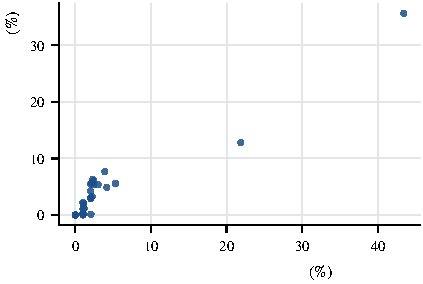
\includegraphics[width=\columnwidth]{fig/fig2_subject_flips.pdf}
\caption{과목별 수정 문항 비율과 라벨 수정 후 결정 반전율($\delta$ = 3\pp{}, 과목마다 861쌍). 점 하나가 한 과목이다.}
\label{fig:subject}
\end{figure}

반전은 수정 문항이 많은 과목에 몰렸다(그림~\ref{fig:subject}). 과목별 반전율과 수정 문항 비율의 상관은 Pearson $r$ = 0.95, Spearman $\rho$ = 0.97이었다. 57과목 중 32과목에서는 반전이 없었다. 바이러스학(virology, 76문항, 수정 문항 비율 43\%)에서는 결정의 36\%가, 대학 화학(college chemistry, 수정 문항 비율 22\%)에서는 13\%가 바뀌었다. 상관은 바이러스학을 빼면 $r$ = 0.81, 대학 화학까지 빼면 $r$ = 0.88로 여전히 높았다.

\subsection{실제 오류는 대표 오답 쪽으로 치우쳤다}

수정 가능 100문항 가운데 43문항에서 원래의 틀린 라벨이 대표 오답과 같았다. 오답 세 개 중 하나를 무작위로 골랐을 때의 기대 일치율 33\%보다 높다(단측 이항검정 $p$ = 0.028, Wilson 95\% 신뢰구간 34--53\%). 같은 문항에서 모델 예측이 원래 라벨과 일치한 비율은 19\%, 수정 라벨과 일치한 비율은 53\%였고, 오류가 없는 문항에서 모델의 평균 정확도는 60\%였다. 실제 오류가 대표 오답 쪽으로 치우친다는 증거는 있으나, 표본이 100건이어서 치우침의 크기는 불확실하다.

\subsection{체계적 오류는 무작위 오류보다 결정을 더 많이 바꾸었다}
\label{sec:injection}

\begin{figure*}[t]
\centering
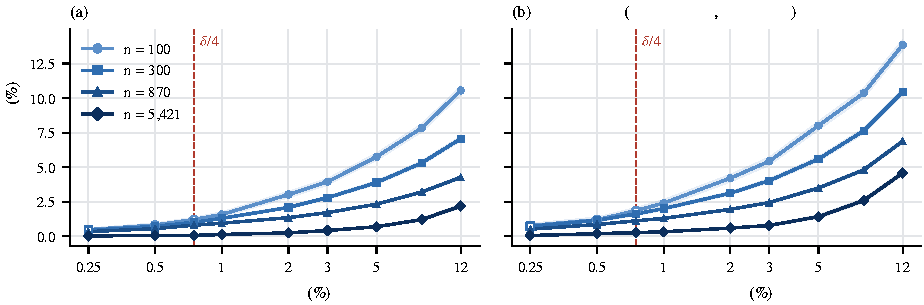
\includegraphics[width=\textwidth]{fig/fig1_flip_vs_error.pdf}
\caption{주입 오류율에 따른 결정 반전율($\delta$ = 3\pp{}, 교차 적합). 띠는 반복 간 95\% 신뢰구간이다. 속이 빈 표식은 기대 오류 문항 수가 1 미만인 조건이며, 점선은 선행 리뷰의 감사 기준 오류율 $\delta/4$ = 0.75\%이다. 가로축은 로그 척도이다.}
\label{fig:injection}
\end{figure*}

\begin{table*}[t]
\centering\small
% generated by app/tables.py from results/; do not edit by hand
\begin{tabular}{@{}lcccccc@{}}
\toprule
 & \multicolumn{4}{c}{라벨 오류} & \multicolumn{2}{c}{기준선(라벨 오류 없음)} \\
\cmidrule(lr){2-5}\cmidrule(l){6-7}
 & 무작위 & 대표 오답 & 어려운 문항 & 체계적 & 문항 교체 & 문항 제거 \\
\midrule
\multicolumn{7}{@{}l}{\textit{결정 반전율(\%)}} \\
$n$ = 100 & 3.94 & 4.65 & 4.46 & 5.43 & 3.39 & 2.32 \\
$n$ = 300 & 2.80 & 3.51 & 3.24 & 4.03 & 2.47 & 1.84 \\
$n$ = 870 & 1.72 & 2.08 & 2.00 & 2.44 & 1.48 & 1.09 \\
$n$ = 5,421 & 0.42 & 0.59 & 0.55 & 0.79 & -- & 0.32 \\
\midrule
\multicolumn{7}{@{}l}{\textit{$n$ = 870에서 반전의 방향(\%)}} \\
결정 상실 & 1.14 & 1.39 & 1.31 & 1.59 & 0.72 & 0.62 \\
허위 결정 & 0.57 & 0.69 & 0.69 & 0.86 & 0.76 & 0.47 \\
\midrule
격차 압축 상관 & −0.86 & −0.80 & −0.68 & −0.46 & −0.01 & 0.01 \\
\bottomrule
\end{tabular}

\caption{오류율 3\%에서 조건별 결정 반전($\delta$ = 3\pp{}, 교차 적합, 반복 300회, 전체 평가셋은 60회). 반전율의 반복 간 95\% 신뢰구간 반폭은 모두 0.3\pp{} 이하이다. 격차 압축 상관은 오류로 생긴 쌍 차이의 변화와 원래 쌍 차이 사이의 Pearson 상관이다($n$ = 870). 전체 평가셋에는 교체할 문항이 남지 않아 문항 교체 기준선을 계산하지 않았다(--).}
\label{tab:injection}
\end{table*}

반전율은 오류율이 높을수록, 평가셋이 작을수록 커졌다(그림~\ref{fig:injection}). 오류율 3\%에서 100문항 평가셋의 반전율은 전체 평가셋의 약 7--9배였다(표~\ref{tab:injection}). 모든 조건에서 역전은 한 건도 없었다.

체계적 오류의 반전율은 무작위 오류의 1.4--1.6배였다(870문항 이하, 오류율 1--5\%, 부트스트랩 신뢰구간 하한 1.28 이상). 전체 평가셋에서는 배율이 1.9--2.5배로 더 컸지만 반전 수가 적어 신뢰구간이 넓었다. 두 요인을 나누어 보면 각 요인이 따로 반전을 늘렸다. 대표 오답 오류는 무작위 오류의 1.2--1.3배, 어려운 문항 오류는 1.1--1.3배였고, 두 요인을 함께 쓴 체계적 오류에서 가장 컸다(표~\ref{tab:injection}).


무작위 라벨 오류의 효과는 라벨 오류가 없는 교란과 크게 다르지 않았다. 870문항 이하에서 무작위 오류의 반전율은 문항 교체 기준선의 1.0--1.2배, 문항 제거 기준선의 1.4--1.7배였다. 체계적 오류의 반전율은 교체 기준선의 약 1.6배였다.

라벨 오류에 고유한 특징은 반전의 방향에서 나타났다. 870문항, 오류율 3\%에서 네 가지 라벨 오류 조건은 모두 결정 상실이 허위 결정의 약 두 배였으나, 교체 기준선에서는 두 방향이 비슷하였다(표~\ref{tab:injection}의 둘째 묶음). 이 비대칭은 격차 압축과 관련된다. 기준 라벨에서 정확도 차이가 큰 쌍일수록 라벨 오류로 차이가 더 많이 줄었다(음의 상관). 오류율 3\%에서 이 상관은 무작위 오류에서 $-0.46$(100문항)부터 $-0.98$(전체 평가셋)까지, 체계적 오류에서 $-0.21$부터 $-0.67$까지였다. 교체 기준선의 상관은 0에 가까웠다($-0.03$에서 $-0.01$).

\subsection{\texorpdfstring{$\delta/4$}{delta/4} 감사 기준 경계의 오류율에서도 결정은 대부분 유지되었다}

\begin{table}[t]
\centering\small\setlength{\tabcolsep}{2.6pt}
% generated by app/tables.py from results/; do not edit by hand
\begin{tabular}{@{}cccccc@{}}
\toprule
 & & \multicolumn{2}{c}{$n$ = 100} & \multicolumn{2}{c}{$n$ = 870} \\
\cmidrule(lr){3-4}\cmidrule(l){5-6}
오류율 & 통과 확률 & 무작위 & 체계적 & 무작위 & 체계적 \\
\midrule
0.25 & 28.0 & 0.48 & 0.78 & 0.34 & 0.51 \\
0.50 & 7.8 & 0.81 & 1.20 & 0.55 & 0.85 \\
0.75 & 2.2 & 1.22 & 1.86 & 0.81 & 1.12 \\
1.00 & 0.6 & 1.58 & 2.40 & 0.94 & 1.30 \\
\bottomrule
\end{tabular}

\caption{509문항 오류 0건 감사의 통과 확률과 같은 오류율에서의 결정 반전율(모두 \%, $\delta$ = 3\pp{}). 통과 확률은 $(1-e)^{509}$이고, 오류율 0.75\%가 $\delta/4$에 해당한다.}
\label{tab:audit}
\end{table}

오류 0건 감사의 95\% Wilson 상한이 $\delta/4$ 이하가 되는 최소 감사 크기는 $\delta$ = 3\pp{}에서 509문항이었다. $\delta$가 1, 2, 5\pp{}이면 각각 1,533, 765, 304문항이다. 따라서 선행 리뷰의 ``509문항 오류 0건'' 규칙은 Wilson 상한 기준과 같은 규칙이다.

표~\ref{tab:audit}는 이 감사의 통과 확률과 같은 오류율에서의 반전율을 함께 보인다. 오류율이 $\delta/4$ = 0.75\%인 평가셋은 2.2\%의 확률로만 감사를 통과한다. 이 오류율에서 870문항 평가셋의 반전율은 무작위 오류 0.81\%, 체계적 오류 1.12\%였고, 문항 교체 기준선은 0.70\%였다. 100문항 평가셋에서는 무작위 오류 1.22\%, 체계적 오류 1.86\%였다. 이 반전의 상당 부분은 문항 교체만으로도 생기는 수준이므로 870문항 이상의 평가셋에서 이 기준은 보수적이지만, 100문항 평가셋에서는 같은 오류율에서도 체계적 오류의 반전율이 1.9\%였다. 통과 확률은 감사의 작동 특성일 뿐이며, 감사를 통과한 평가셋의 오류율 분포는 사전분포 없이 말할 수 없다.

\section{선행 연구 결과와의 비교}
\label{sec:compare}

\begin{table*}[t]
\centering\small\setlength{\tabcolsep}{4pt}
% generated by app/tables.py from results/; do not edit by hand
\begin{tabular}{@{}>{\raggedright\arraybackslash}p{2.0cm}>{\raggedright\arraybackslash}p{4.6cm}>{\raggedright\arraybackslash}p{3.6cm}>{\raggedright\arraybackslash}p{4.7cm}@{}}
\toprule
선행 연구 & 비교 항목 & 보고값 & 본 연구의 대응 값 \\
\midrule
\citet{gema-etal-2025-done} & MMLU 오류 문항 비율(층화 추정) & 6.49\% & 논문 표 5로 재계산 6.49\%, 배포 자료 6.48\%(판단 유보 32문항 포함 시 7.00\%) \\
 & 바이러스학을 오류 없는 문항으로만 채점할 때의 순위 변화 & Llama 3.1 405B가 HELM 16위에서 10개 모델 중 공동 1위로 & 최대 14계단, $\tau$ = 0.76. 같은 수의 문항을 무작위로 뽑아도 최대 20계단, $\tau$ = 0.68 \\
 & 과목 정확도와 오류 없는 문항 비율의 모델별 상관 & $r$ = 0.33--0.54 & $r$ = −0.18--0.31(중앙값 0.16) \\
\midrule \citet{vendrow2025platinum} & 모델 오답 가운데 벤치마크 오류가 차지하는 몫 & MMLU 고교 수학 5\%, 벤치마크 14종 0--93\% & 고교 수학 0\%, MMLU 전체 7.4\%(상위 5종 10.4\%), 바이러스학 57\% \\
\midrule \citet{northcutt2021pervasive} & 수정 가능한 오류 문항의 비율 $N_0$ & ImageNet 2.9\%, CIFAR-10 0.2\% & 1.84\%(100/5,421) \\
 & 오류 문항 비율을 6\%p 높일 때 수정 라벨에서 순서가 바뀌는 쌍(원래 비율 대비) & ImageNet에서 ResNet-18과 ResNet-50의 순서가 바뀜 & 861쌍 중 3쌍 \\
 & 수정 가능 문항에서 원래 라벨 순위와 수정 라벨 순위의 관계 & 음의 관계(NASNet-large 1위에서 29위) & Spearman $\rho$ = −0.58 \\
 & 전체 성능이 높은 모델이 원래의 틀린 라벨을 고르는 경향 & 고용량 모델일수록 강함 & 반대 방향, Spearman $\rho$ = −0.43 \\
\midrule \citet{madaan2024variance} & 100문항 부분셋에서 전체 평가셋과 순서가 바뀌는 쌍(그들은 IRT로 선택, 본 연구는 무작위) & 4.5--12.2\% & 무작위 100문항 7.8\%, 과목 단위 라벨 수정 0.7\% \\
 & MMLU 정확도의 학습 시드 표준편차 & 0.57\%p & 라벨 수정에 따른 정확도 변화 평균 0.63\%p, 쌍 차이 변화 중앙값 0.18\%p \\
\midrule \citet{card-etal-2020-little} & 검정력 80\%의 최소 검출 효과 & 147문항 5.26\%p, 5,463문항 0.55\%p & 100문항 14.6\%p, 5,421문항 2.0\%p(쌍별 중앙값) \\
\midrule \citet{alzahrani-etal-2024-benchmarks} & 순위가 바뀐 모델의 수와 최대 이동 폭 & MMLU 세 과목의 답 순서 섞기에서 11종 중 5종, 여러 교란에서 최대 8계단 & 라벨 수정에서 42종 중 6종, 최대 2계단 \\
\bottomrule
\end{tabular}

\caption{선행 연구의 보고값과 본 연구의 자료(모델 42종, MMLU-Redux 2.0)에서 재현하거나 계산한 대응 값. 보고값은 각 논문의 본문, 표, 그림에서 옮겼다. 보고값과 본 연구 값은 모델과 과제가 다르므로, 수치의 차이에는 절차 외의 차이도 들어 있다.}
\label{tab:compare}
\end{table*}

표~\ref{tab:compare}는 선행 연구가 보고한 값과 본 연구의 자료에서 재현하거나 계산한 대응 값을 나란히 보인다. 이 절에서는 외부 예측의 재현을 먼저 확인하고, 일치한 결과와 어긋난 결과를 차례로 살핀다.

\subsection{리더보드 예측은 로컬 재실행으로 재현되었다}

\begin{table}[t]
\centering\small\setlength{\tabcolsep}{3.5pt}
% generated by app/tables.py from results/; do not edit by hand
\begin{tabular}{@{}lccc@{}}
\toprule
 & 예측 일치 & 로그우도 & 수정 후 변화(\%p) \\
모델 & (\%) & 차이 & 리더보드, 재실행 \\
\midrule
phi-2 & 99.2 & 0.012 & 0.65, 0.65 \\
Mistral-7B-v0.1 & 99.8 & 0.001 & 0.89, 0.89 \\
stablelm-3b-4e1t & 99.5 & 0.003 & 0.70, 0.70 \\
\bottomrule
\end{tabular}

\caption{리더보드 예측과 로컬 재실행 예측(5,690문항, float16, Apple 실리콘 GPU). 예측 일치는 로그우도가 가장 큰 선택지가 같은 문항의 비율, 로그우도 차이는 네 선택지 로그우도 차이의 절댓값 중앙값이다. 수정 후 변화는 $S$에서 수정 정답과 원래 정답 기준 정확도의 차이이다.}
\label{tab:rerun}
\end{table}

세 모델을 다시 실행한 예측은 리더보드 예측과 문항의 99.2--99.8\%에서 일치하였다(표~\ref{tab:rerun}). 예측이 갈린 문항에서 리더보드의 상위 두 선택지 로그우도 차이는 중앙값 0.016 이하로, 사실상 동점인 문항이었다. 라벨 수정에 따른 정확도 변화는 두 예측에서 소수점 둘째 자리까지 같았고, 세 모델 쌍의 판정도 원래 라벨과 수정 라벨 모두에서 같았다. phi-2는 공통 앞부분을 재사용하지 않고 문항마다 전체를 계산한 실행과도 로그우도가 완전히 같았다. 가중치 판과 실행 환경이 달라도 외부 예측은 결론을 바꿀 만큼 다르지 않았다.

\subsection{MMLU-Redux의 오류율은 재현되었으나, 보고된 순위 변화는 문항 수의 효과와 구별되지 않았다}

\citet{gema-etal-2025-done}의 과목별 표로 층화 추정치를 다시 계산하면 보고값과 같은 6.49\%가 나왔다. 배포된 자료로는, 주석자가 더 많은 전문 지식이 필요하다며 판단을 유보한 expert 유형 32문항을 빼면 6.48\%, 오류로 세면 7.00\%였다. 57과목 중 46과목은 유형별 문항 수가 표와 같았고, 고교 수학에서는 표의 정답 오류 1건이 배포 자료에 없었다. \citet{vendrow2025platinum}의 연구도 이 과목에서 Redux 주석자가 맞는 정답을 틀리게 고친 문항 하나를 보고하였다.

그들의 표 2는 HELM의 전체 문항 점수에 따른 순위와 Redux의 오류 없는 문항 점수에 따른 10개 모델 사이의 순위를 비교하였고, 바이러스학의 Llama 3.1 405B는 HELM 16위에서 공동 1위가 되었다. 표 제목은 전체 문항 점수를 HELM에서 가져왔다고 쓰지만 본문(5쪽)은 MMLU-Redux의 모든 문항이라고 써서 해석이 갈린다. 표 제목을 따라 같은 비교를 모델 42종에 적용하면, 바이러스학에서 순위가 최대 14계단 움직였다($\tau$ = 0.76). 그러나 라벨과 무관하게 MMLU 전체 문항에서 같은 수(43문항)를 무작위로 뽑기만 해도 순위는 최대 20계단 움직였다($\tau$ = 0.68, 200회의 중앙값). 57과목 평균으로 순서가 바뀐 쌍은 그들의 비교에서 4.7\%, 무작위 대조에서 4.4\%였다. Redux 100문항에서 오류 문항을 빼는 단계만 보아도 0.84\%로, 같은 수의 문항을 무작위로 뺄 때(0.84\%)와 같았다. 따라서 오류 문항을 빼고 채점하는 비교로는 라벨 오류의 효과를 문항 수가 줄어드는 효과와 구별하기 어렵다. 라벨만 바꾸는 본 연구의 비교에서는 바이러스학의 순위가 최대 18계단 움직여($\tau$ = 0.60), 오류가 몰린 과목에서는 라벨 오류 자체도 순위를 크게 바꾸었다.

과목별 정확도와 오류 없는 문항 비율의 상관이 그들의 보고보다 약했던 것은 모델의 성능 수준과 관련된 것으로 보인다. 이 상관은 모델의 전체 정확도와 함께 커졌고(Spearman $\rho$ = 0.87), 상위 10종의 중앙값은 0.25, 하위 10종은 0.04였다. 정확도가 낮은 모델의 오답은 대부분 난도에서 오므로 라벨 오류의 몫이 작다.

\subsection{이미지 분류와 달리, 강한 모델은 오류 문항에서 수정 정답을 더 자주 골랐다}
\label{sec:capacity}

\citet{northcutt2021pervasive}의 절차로 오류 문항의 비율을 6\%p 높여도(1,275문항) 수정 라벨에서의 순서가 원래 비율일 때와 달라진 쌍은 861쌍 중 3쌍이었고, 원래 라벨과 수정 라벨의 순서가 다른 쌍은 8쌍이었다. 수정 라벨에서 순서가 언젠가 바뀌는 136쌍 가운데 절반은 오류 문항이 70\% 이상일 때 바뀌었다. 줄인 평가셋에 본 연구의 결정 규칙을 적용하면 원래 라벨과 수정 라벨 사이의 결정 반전율은 $N_0$에서 0.9\%, 7.84\%에서 2.4\%, 20\%에서 7.1\%였다. 역전은 오류 문항이 절반인 200문항 평가셋에서만 나타났고, 172,200회의 판정 중 6건이었다.

어긋난 것은 모델 용량과 틀린 라벨의 관계이다. 수정 가능 문항에서 원래 라벨 기준 순위와 수정 라벨 기준 순위가 반대 방향이라는 점은 같았다(Spearman $\rho$ = $-0.58$). 그러나 그들의 자료에서는 고용량 모델이 원래 라벨로 잘한 반면, 본 연구에서는 약한 모델이 원래 라벨로 잘하였다($\rho$ = $-0.43$). 정확도 상위 10종은 수정 정답을 62.4\%, 틀린 라벨을 16.8\% 골랐고, 하위 10종은 각각 37.2\%와 23.1\% 골랐다. 차이는 주로 강한 모델이 수정 정답을 더 자주 고른 데서 왔다. 틀린 답만 보면 원래 라벨을 고른 비율은 오히려 상위 10종에서 높았다(44.7\% 대 36.3\%). 이미지 분류에서는 라벨 오류가 고용량 모델에 유리하였지만 본 연구에서는 강한 모델에 불리하였고, \ref{sec:natural}절과 \ref{sec:injection}절의 격차 압축과 결정 상실은 이 방향에서 나온다. \citet{gema-etal-2025-done}이 오류 문항 암기의 근거로 든 양상, 즉 오류 문항의 정확도가 오류 없는 문항과 비슷하거나 높은 현상은 그들이 든 전문 법학과 형식 논리에서 본 연구의 상위 10종에도 나타났다(오류 문항 18개와 13개). 그러나 과목을 합치면 미해결 문항의 원래 정답을 맞힌 비율(57.3\%)은 오류 없는 문항(73.6\%)보다 낮았다.

\subsection{전체 평가셋에서 라벨 오류는 다른 평가 잡음보다 작았다}

과목 단위에서 라벨 수정이 순서를 바꾼 쌍(평균 0.7\%)은 무작위 100문항 표본이 바꾼 쌍(7.8\%)의 약 10분의 1이었다. 라벨 수정에 따른 정확도 변화(평균 0.63\%p)는 \citet{madaan2024variance}가 우연 수준의 7B 모델에서 보고한 MMLU 학습 시드 표준편차(0.57\%p)와 비슷하였지만, 결정에 쓰이는 쌍 차이의 변화는 중앙값 0.18\%p로 쌍 차이의 표준오차 중앙값 0.71\%p보다 작았다. 순위 변화도 \citet{alzahrani-etal-2024-benchmarks}가 보고한 평가 형식 교란의 효과보다 작았다.

최소 검출 효과는 \citet{card-etal-2020-little}의 보고보다 훨씬 컸다. 그들의 과제는 정확도가 90\%를 넘어 두 모델의 정오가 엇갈리는 문항이 적지만, MMLU의 모델 쌍은 문항의 29\%(중앙값)에서 정오가 엇갈렸다. 선행 리뷰는 이 비율을 0.10으로 가정하여 870문항을 권하였으나, MMLU 같은 과제에서 870문항의 최소 검출 효과(4.9\%p)는 $\delta$ = 3\pp{}보다 크다.

\section{논의}

\paragraph{라벨 오류는 주로 결정을 보류로 바꾼다.}
4지선다 문항을 정확도로 채점할 때 라벨 오류는 해당 문항을 맞힌 모델의 점수를 깎고, 오류 라벨과 같은 오답을 고른 모델에 점수를 준다. 정확도가 높은 모델일수록 깎이는 문항이 많으므로 격차가 줄고, 반전은 결정 상실 쪽으로 치우친다. 실제 오류 수준과 주입 실험의 범위에서 우세 방향이 뒤집힌 경우는 없었고, 대신 작은 차이를 가려낼 검정력이 줄었다. 따라서 라벨 오류의 주된 비용은 잘못된 모델 선택보다 판정 보류와 그에 따른 추가 평가에 있을 가능성이 크다. 이 방향은 강한 모델이 오류 문항에서 수정 정답을 더 자주 고르기 때문에 생긴다(\ref{sec:capacity}절). 골든셋의 라벨을 모델로 생성한 경우에는 오류가 그 모델과 비슷한 후보의 예측 쪽으로 치우칠 수 있으므로, 이때는 본 연구의 결과를 그대로 적용하기 어렵다.

\section{결론}

실제 오류 수준에서 골든셋 라벨 오류는 모델 순위를 거의 바꾸지 않았고, 모델 간 격차를 줄여 결정을 보류로 바꾸었다. 체계적 오류는 무작위 오류보다 약 1.5배 큰 효과를 냈고, 효과는 작은 평가셋과 오류가 몰린 과목에서 컸다. 선행 연구와 비교하면 오류 문항을 빼는 비교는 문항 수의 효과와 구별되지 않았고, 강한 LLM은 이미지 분류와 달리 오류 문항에서 수정 정답을 더 자주 골랐다. 허용 오류율은 체계적 오류 기준으로 정하고, 하위 집합마다 오류율을 감사하며, 평가셋 크기는 실제 모델 쌍의 정오 엇갈림 비율로 정할 것을 권한다.
\label{sec:end-of-body}

\section*{한계}

\paragraph{과제와 채점.}
MMLU는 4지선다 정확도 과제이다. 생성형 응답이나 RAG 출력을 판정 모델로 채점하는 평가에서는 라벨 오류가 격차를 압축하지 않을 수 있다.

\paragraph{모델.}
MMLU 문항별 결과가 공개된 2023--2024년 모델로 한정되며, Llama-2 chat 같은 공식 대화형 모델이 빠졌다. 최신 모델에서의 결과는 확인하지 않았다.

\paragraph{라벨.}
미해결 오류 269문항은 기준 라벨에서 제외하였고, Redux 재주석 자체의 오류는 고려하지 않았다. 실제 오류의 체계성 추정(RQ2)은 100건에 기반한다.

\paragraph{선행 연구와의 비교.}
보고값은 다른 모델과 과제(이미지 분류, 다른 벤치마크, HELM의 모델)에서 나온 값이므로, 같은 분석을 재현하더라도 수치의 차이에는 모델과 과제의 차이가 함께 들어 있다. 로컬 재실행은 세 모델에 한정되며, 가중치 판이 리더보드의 실행 시점과 다를 수 있다.

\paragraph{결정 규칙과 측정 범위.}
결과는 결정 규칙에 의존하며, McNemar--Holm 규칙에서 과목 단위 반전은 절반 이하로 줄었다. 반전율은 같은 표본 안의 교란 효과만 측정하며, 표본 추출 변동에 따른 결정의 불안정은 다루지 않았다.

\bibliography{references}

\appendix

\section{모델 목록}
\label{app:models}

표~\ref{tab:models}은 분석에 포함한 모델 42종과 세 라벨 조건에서의 정확도를 보인다. 모델 이름은 Hugging Face 저장소 이름이다. 제외한 6종 가운데 \texttt{allenai/OLMo-7B}, \texttt{deepseek-ai/deepseek-llm-7b-base}, \texttt{internlm/internlm2-7b}는 추정한 이름의 리더보드 저장소가 없었다. Llama-2 chat 3종(7B, 13B, 70B)은 리더보드 저장소에 MMLU 문항별 결과가 없었다. OLMo 2종을 추가하기 전의 40종으로 분석한 결과도 본문의 결론과 같았다.

\begin{table*}[t]
\centering\small
% generated by app/tables.py from results/; do not edit by hand
\begin{tabular}{@{}lrrrr@{}}
\toprule
모델 & 공개 점수 & $S$ 원래 정답 & $S$ 수정 정답 & 변화(\%p) \\
\midrule
\texttt{Qwen/Qwen1.5-72B} & 77.3 & 78.0 & 78.9 & 0.87 \\
\texttt{01-ai/Yi-34B} & 76.1 & 76.8 & 77.6 & 0.79 \\
\texttt{NousResearch/Nous-Hermes-2-Mixtral-8x7B-DPO} & 72.0 & 72.8 & 73.6 & 0.79 \\
\texttt{mistralai/Mixtral-8x7B-v0.1} & 71.9 & 72.6 & 73.5 & 0.81 \\
\texttt{deepseek-ai/deepseek-llm-67b-base} & 71.9 & 72.6 & 73.4 & 0.85 \\
\texttt{mistralai/Mixtral-8x7B-Instruct-v0.1} & 71.3 & 71.9 & 72.8 & 0.96 \\
\texttt{tiiuae/falcon-180B} & 70.6 & 71.2 & 72.0 & 0.87 \\
\texttt{meta-llama/Llama-2-70b-hf} & 70.0 & 70.6 & 71.4 & 0.77 \\
\texttt{Qwen/Qwen1.5-14B} & 69.4 & 70.4 & 71.2 & 0.79 \\
\texttt{Qwen/Qwen-14B} & 67.7 & 68.5 & 69.4 & 0.90 \\
\texttt{meta-llama/Meta-Llama-3-8B-Instruct} & 67.2 & 68.0 & 68.8 & 0.85 \\
\texttt{meta-llama/Meta-Llama-3-8B} & 67.2 & 67.7 & 68.5 & 0.81 \\
\texttt{google/gemma-7b} & 66.0 & 66.6 & 67.3 & 0.74 \\
\texttt{upstage/SOLAR-10.7B-v1.0} & 65.2 & 65.9 & 66.7 & 0.87 \\
\texttt{openchat/openchat\_3.5} & 65.2 & 65.9 & 66.5 & 0.61 \\
\texttt{WizardLM/WizardLM-70B-V1.0} & 64.8 & 65.3 & 65.9 & 0.65 \\
\texttt{huggyllama/llama-65b} & 64.3 & 64.7 & 65.4 & 0.68 \\
\texttt{mistralai/Mistral-7B-v0.1} & 63.7 & 64.3 & 65.2 & 0.89 \\
\texttt{teknium/OpenHermes-2.5-Mistral-7B} & 63.7 & 64.4 & 65.1 & 0.66 \\
\texttt{01-ai/Yi-6B} & 63.6 & 64.4 & 65.1 & 0.70 \\
\texttt{Qwen/Qwen1.5-7B} & 62.3 & 62.8 & 63.5 & 0.72 \\
\texttt{HuggingFaceH4/zephyr-7b-beta} & 61.2 & 61.7 & 62.6 & 0.87 \\
\texttt{mistralai/Mistral-7B-Instruct-v0.2} & 61.1 & 61.8 & 62.5 & 0.70 \\
\texttt{Intel/neural-chat-7b-v3-1} & 60.5 & 61.3 & 62.1 & 0.81 \\
\texttt{Qwen/Qwen-7B} & 59.7 & 60.3 & 61.0 & 0.72 \\
\texttt{huggyllama/llama-30b} & 58.3 & 58.9 & 59.7 & 0.81 \\
\texttt{microsoft/phi-2} & 58.2 & 58.6 & 59.2 & 0.65 \\
\texttt{tiiuae/falcon-40b} & 57.0 & 57.8 & 58.3 & 0.57 \\
\texttt{lmsys/vicuna-13b-v1.5} & 57.0 & 57.7 & 58.2 & 0.52 \\
\texttt{meta-llama/Llama-2-13b-hf} & 54.5 & 55.0 & 55.6 & 0.63 \\
\texttt{allenai/OLMo-1.7-7B-hf} & 53.6 & 54.2 & 54.7 & 0.50 \\
\texttt{lmsys/vicuna-7b-v1.5} & 51.2 & 51.7 & 52.4 & 0.68 \\
\texttt{huggyllama/llama-13b} & 47.9 & 48.5 & 49.0 & 0.52 \\
\texttt{mosaicml/mpt-30b} & 47.7 & 48.1 & 48.6 & 0.57 \\
\texttt{meta-llama/Llama-2-7b-hf} & 46.8 & 47.2 & 47.7 & 0.50 \\
\texttt{stabilityai/stablelm-3b-4e1t} & 45.1 & 45.5 & 46.2 & 0.70 \\
\texttt{google/gemma-2b} & 42.9 & 43.5 & 43.7 & 0.28 \\
\texttt{huggyllama/llama-7b} & 36.4 & 36.7 & 36.9 & 0.18 \\
\texttt{mosaicml/mpt-7b} & 31.1 & 31.0 & 31.0 & −0.04 \\
\texttt{allenai/OLMo-7B-hf} & 27.9 & 28.0 & 28.0 & 0.00 \\
\texttt{tiiuae/falcon-7b} & 27.3 & 27.6 & 27.4 & −0.11 \\
\texttt{EleutherAI/pythia-12b} & 27.5 & 27.4 & 27.4 & 0.00 \\
\bottomrule
\end{tabular}

\caption{모델별 정확도(\%). 공개 점수는 결합된 5,690문항의 원래 정답, $S$ 원래 정답과 $S$ 수정 정답은 분석 집합 5,421문항에서의 정확도이며, 변화는 수정 정답과 원래 정답의 차이이다. 수정 정답 기준 정확도 순으로 정렬하였다.}
\label{tab:models}
\end{table*}

\section{실험 세부 사항}
\label{app:details}

\paragraph{문항 결합.}
Redux 문항의 질문과 네 선택지를 lm-evaluation-harness의 MMLU 프롬프트 형식(질문, A--D 선택지, ``Answer:'')으로 이어 붙이고 연속된 공백을 하나로 정규화하였다. 리더보드 상세 파일의 문항 필드도 같은 방식으로 정규화한 뒤, 과목명과 함께 결합 키로 사용하였다. 모든 모델의 예측이 있는 문항만 남겼다.

\paragraph{오류 주입.}
오답률 비례 추출의 가중치는 다른 집단 모델의 문항별 오답률에 0.001을 더한 값이다. 모든 모델이 맞힌 문항의 대표 오답은 세 오답 중 하나를 무작위로 정하였다. 한 반복은 두 집단에서 210쌍씩 모두 420쌍을 평가한다. 반복 간 신뢰구간은 반복별 반전율의 평균에 표준오차의 1.96배를 더하고 뺀 구간이다. 조건 간 배율의 신뢰구간은 반복을 복원 추출하여 두 조건의 평균 반전율의 비를 1,000회 계산한 뒤 2.5와 97.5 백분위수로 구하였다.

\paragraph{난수 시드.}
모델 분할에 7, 표본 추출과 오류 주입에 42, 부트스트랩에 1, 대표 오답의 무작위 보조 추첨에 0을 사용하였다.

\paragraph{재현.}
코드와 결과 파일은 공개 저장소의 \texttt{app/}과 \texttt{results/}에 있다. \texttt{fetch.py}가 데이터를 내려받고, \texttt{analyze.py}가 결과 파일을, \texttt{figures.py}와 \texttt{tables.py}가 그림과 표를 만든다. 선행 연구의 재현은 \texttt{compare.py}가, 로컬 재실행은 \texttt{rerun\_local.py}가 수행한다. 비교에 쓴 선행 연구의 보고값은 출처 쪽수와 함께 \texttt{reference\_numbers.py}에 모았다. MMLU-Redux 2.0은 CC BY 4.0으로 배포되며, 원자료는 저장소에 복사하지 않았다.

\end{document}
